\subsection{Systematic uncertainties}

\tk{TODO:
Treat here how the scale variations are used, and explain the procedure to implement the bin-to-bin correlations in the likelihood.
% 
Note PDF uncertainties are not included.
% 
Refer back to this section for the kb/kc fits.
}

The theoretical predictions described in Section~\ref{sec:theory} are subject to theoretical uncertainties from the renormalisation scale $\muR$ and the factorisation scale $\muF$.
% 
The standard approach to evaluate the impact of these uncertainties is to compute an envelope of scale variations, and to assign the extrema of the envelope as the uncertainty.
% 
To this end, $\muR$ and $\muF$ are independently varied between $0.5$, $1$, and $2$ times their nominal value, whereas the fraction $\frac{\muR}{\muF}$ is constrained not to be less than $0.5$ or greater than $2.0$.
% 
As the theoretical spectra in the $\kappat$/$\cg$/$\kappab$ case and the $\kappac$/$\kappab$ case contain a resummation, the uncertainty in the resummation scale $Q$ is also considered, and it is evaluated by varying $Q$ from $0.5$ to $2$ times its central value (while keeping $\muF$ and $\muR$ at their respective central values).
% 
The theoretical uncertainties are assigned by applying the minimum and maximum scale variations per bin.
% 
The resulting uncertainties for the spectra under variations of $\kappab$ and $\kappac$ and variations of $\kappat$, $\cg$, and $\kappab$ are shown in Table~\ref{tab:TheoryUncertainties_kappab_kappac} and \ref{tab:TheoryUncertainties_kappat_kappag}, respectively.


\begin{table}[htb]
\caption{
    Theoretical uncertainties in the transverse momentum spectra under variations of $\kappab$ and $\kappac$.
    }
\label{tab:TheoryUncertainties_kappab_kappac}
\footnotesize
\begin{center}
\begin{tabular}{lccccc}
\hline
% Generated on 18-05-04 16:59:22 by differentials/theory/scalecorrelation.py; current git commit: e4def5d final versions of fermilab plots
Binning (GeV) & [0, 15) & [15, 30) & [30, 45) & [45, 80) & [80, 120) \\
$\Delta^\text{scale}$ (\%) & 8.9\% & 6.6\% & 18.1\% & 22.0\% & 21.6\% \\
\hline
\end{tabular}
\end{center}
\end{table}

\begin{table}[htb]
\caption{
    Theoretical uncertainties in the transverse momentum spectra under variations of $\kappat$, $\cg$, and $\kappab$.
    }
\label{tab:TheoryUncertainties_kappat_kappag}
\footnotesize
\begin{center}
\setlength{\tabcolsep}{2pt}
\begin{tabular}{lccccccccc}
\hline
% Generated on 18-05-04 16:59:21 by differentials/theory/scalecorrelation.py; current git commit: e4def5d final versions of fermilab plots
Binning (GeV) & [0, 15) & [15, 30) & [30, 45) & [45, 80) & [80, 120) & [120, 200) & [200, 350) & [350, 600) & [600, 800) \\
$\Delta^\text{scale}$ (\%) & 12.7\% & 7.4\% & 9.5\% & 12.8\% & 17.4\% & 19.3\% & 20.9\% & 23.4\% & 8.2\% \\
\hline
\end{tabular}
\end{center}
\end{table}


Theoretical uncertainties are subject to bin-to-bin correlations.
% 
We adopt a procedure that produces a correlation coefficient $\rho_{ab}$ directly from the individual scale variations:
% 
\begin{linenomath*}
\begin{equation}
\rho_{ab} = 
\frac{
    \sum_i ( \sigma_{a, i} - \overline{\sigma}_a ) ( \sigma_{b, i} - \overline{\sigma}_b )
    }{
    \sqrt{
        \sum_i ( \sigma_{a, i} - \overline{\sigma}_a )^2
        \sum_i ( \sigma_{b, i} - \overline{\sigma}_b )^2
        }
    }
    \,,
\end{equation}
\end{linenomath*}
% 
where $\sigma_{a (b), i}$ is the cross section in bin $a$ ($b$) of the $i^\text{th}$ scale variation, $\overline{\sigma}_{a (b)}$ is the mean cross section in bin $a$ ($b$), and $\rho_{ab}$ is the resulting correlation coefficient between bin $a$ and $b$.
% 
The correlation structure is characterized by strong correlations among bins at moderate transverse momentum ($15 \leq \pth \leq 600\GeV$).
% 
Only the bins with $\pth<15$ and $\pth>600$\GeV are anti-correlated with the bins at moderate transverse momentum.

The correlation matrices obtained from this procedure are shown in Fig.~\ref{fig:scalecorrelationmatrices}.
% 
In both cases the low $\pth$-region is less correlated with other bins than the other bins among one another.
% 
This is mostly due to the resummation that has a large impact on the low $\pth$-region.
% 
In the case of $\kappat$/$\cg$ variations, the overflow bin is less correlated as well.


\begin{figure}[hbtp]
  \begin{center}
    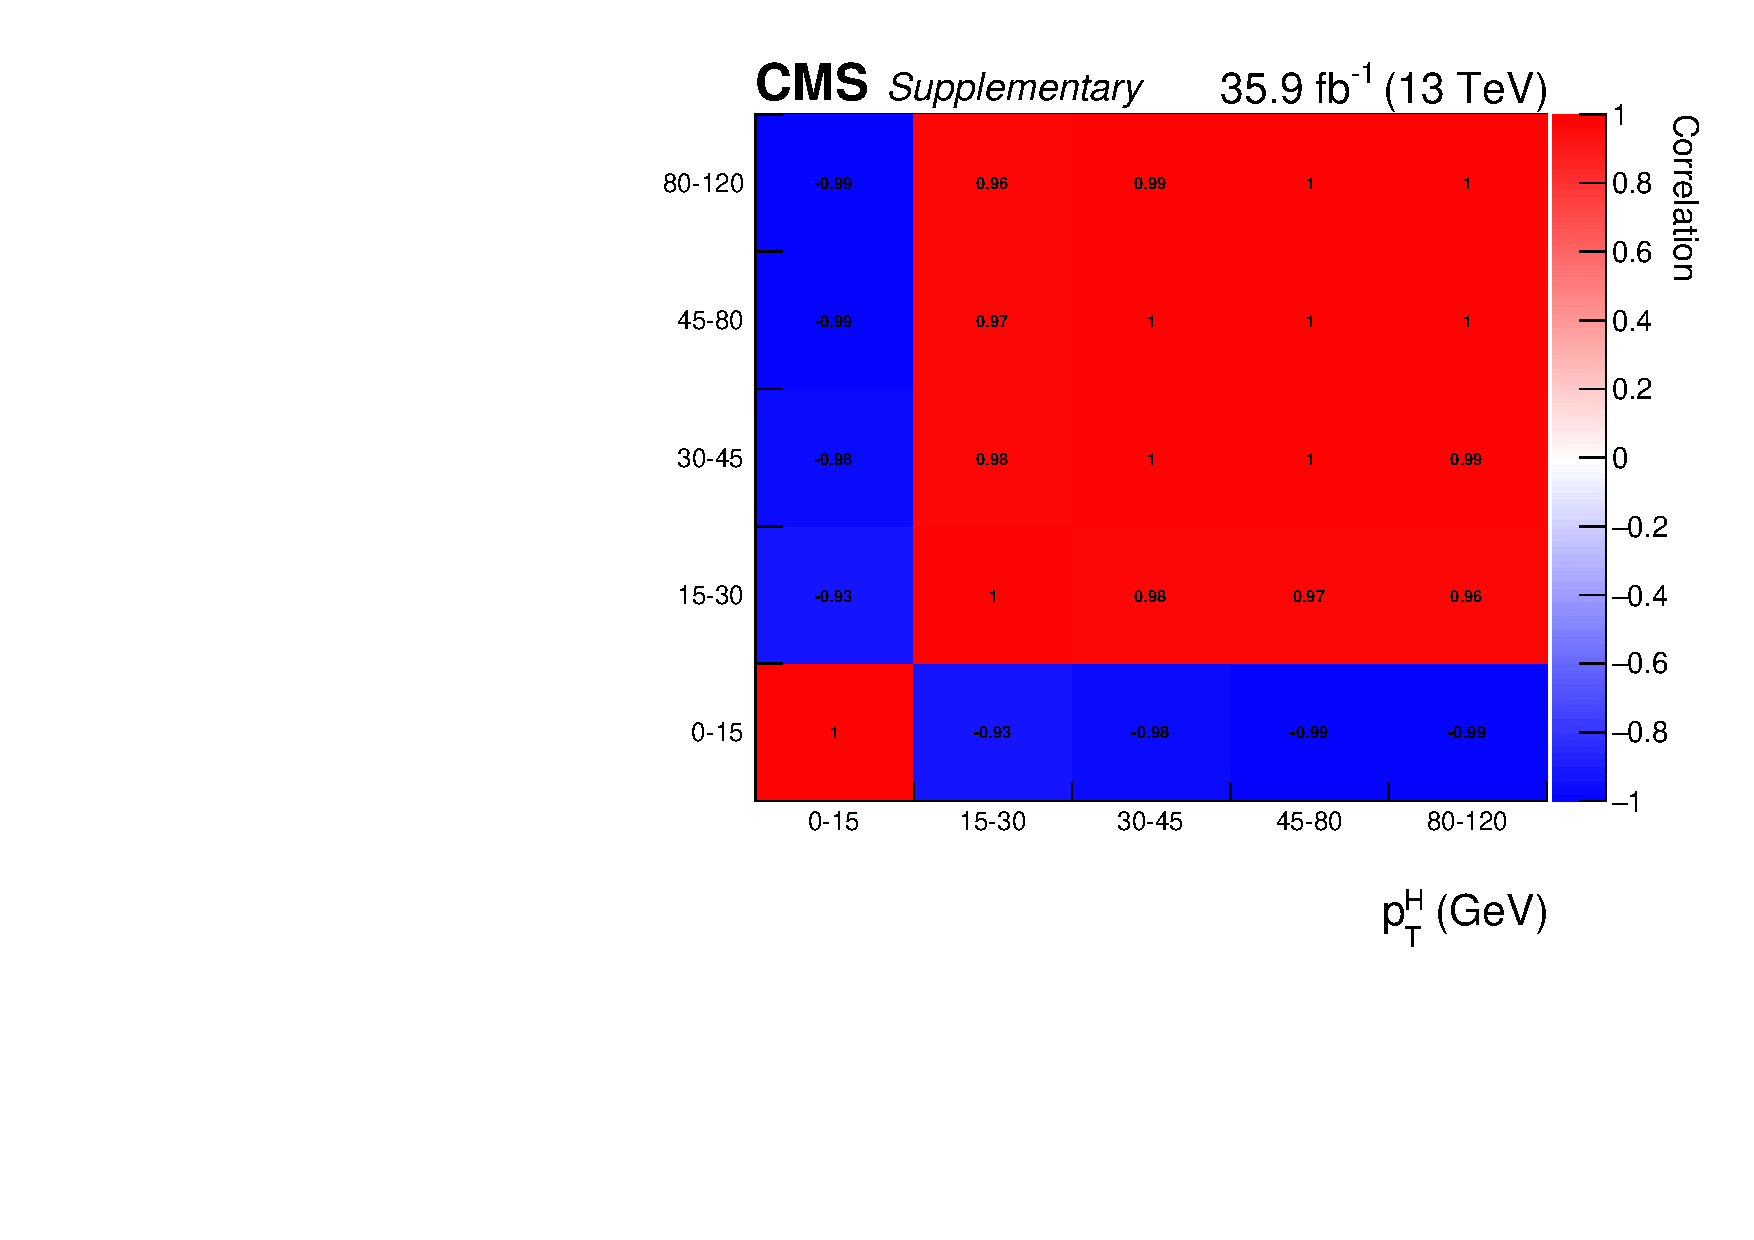
\includegraphics[width=\halflinewidth]{img/interpretation/other/corrmat_yukawa.pdf}
    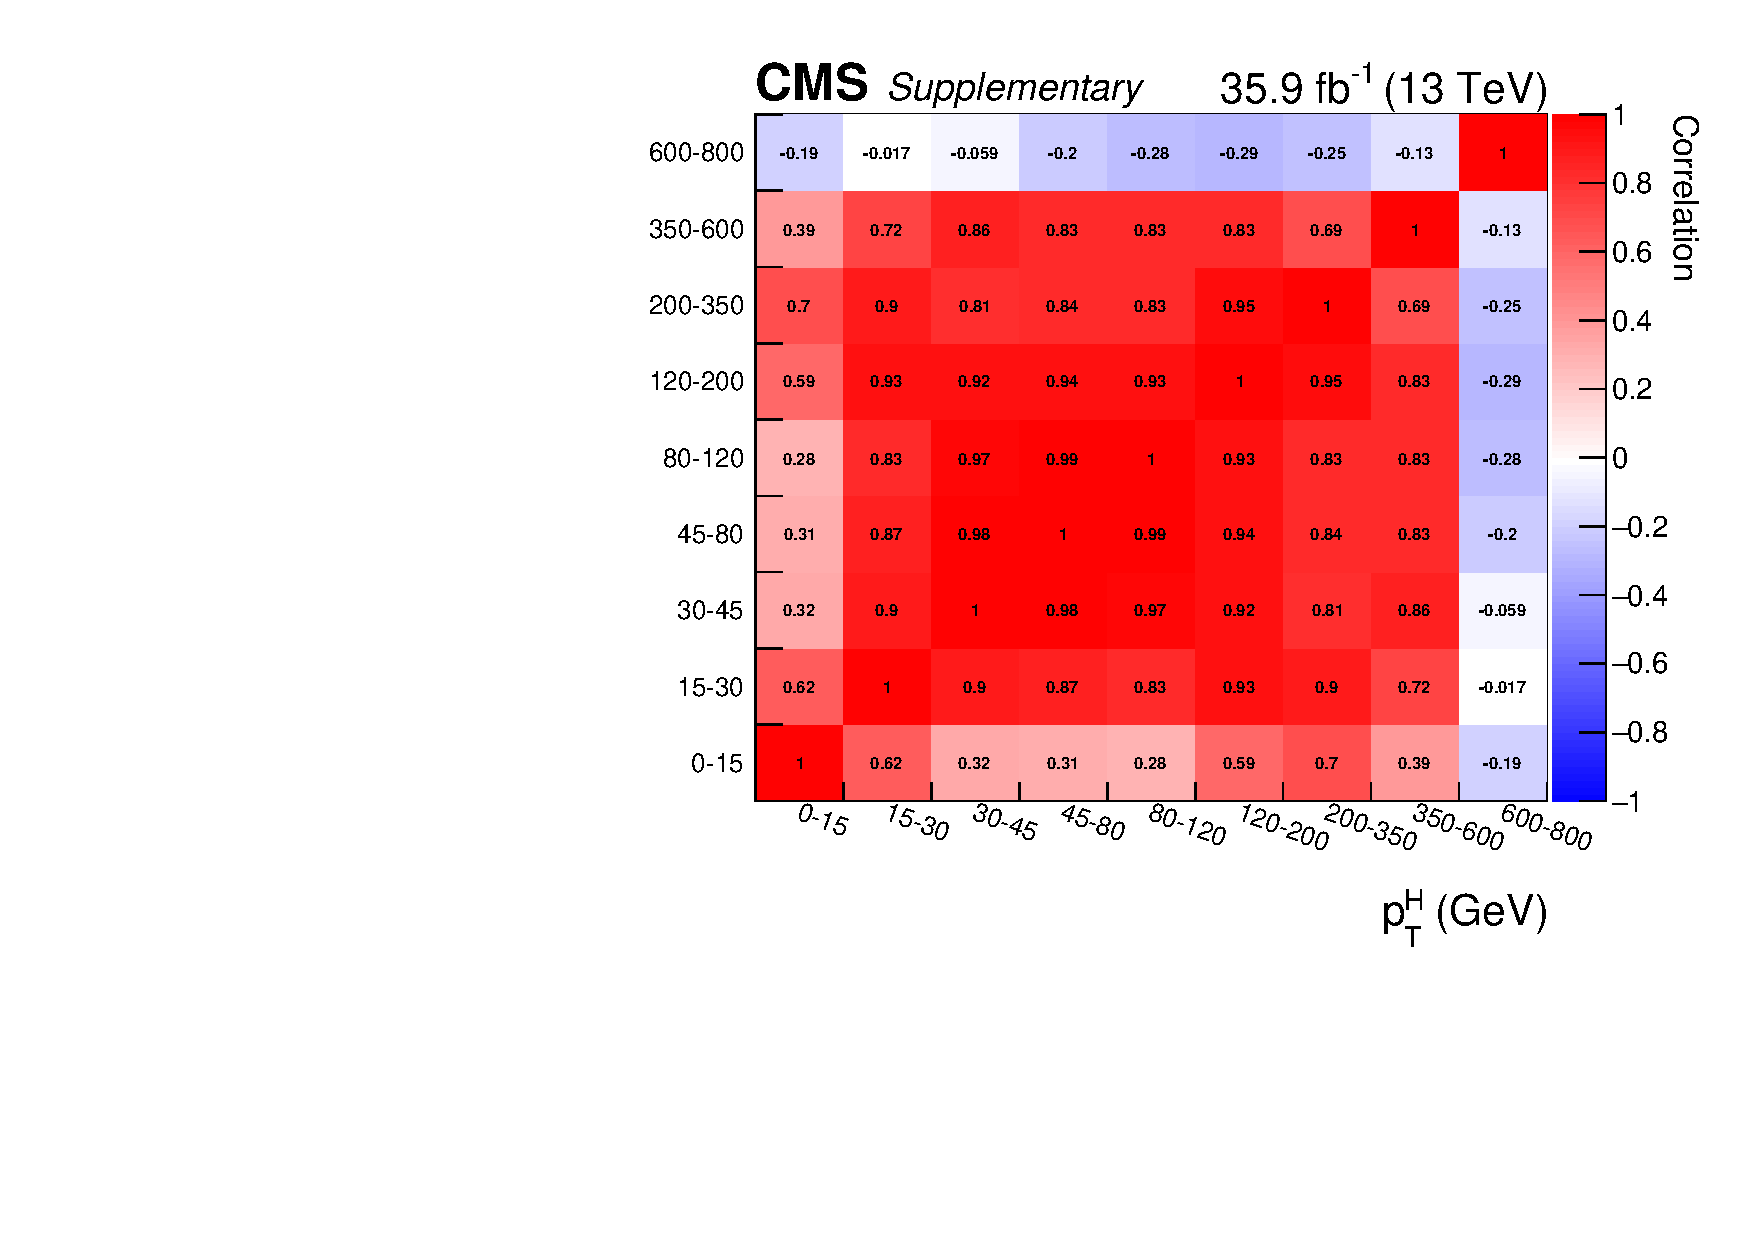
\includegraphics[width=\halflinewidth]{img/interpretation/other/corrmat_tophighpt.pdf}
    \caption{
        (left) Correlation matrix for theoretical uncertainties on $\kappab$/$\kappac$ variations.
        (right) Correlation matrix for theoretical uncertainties on $\kappat$/$\cg$/$\kappab$ variations.
        }
    \label{fig:scalecorrelationmatrices}
  \end{center}
\end{figure}


\tk{Scale uncertainty implementation in combine (doing the PCA, adding as nuis pars) -- should it go in?}


\subsubsection{Dependence of the correlation matrix on the couplings}

The procedure described in Sec.~\ref{sec:correlationmatrixprocedure} neglects the effect of coupling variations on the correlation matrix.
% 
In order to estimate the impact of this effect, the correlation matrices in Sec.~\ref{sec:correlationmatrixresults} are computed at different values of the couplings $\kappa_b$ and $\kappa_c$, using only the gluon-induced contributions (because only of only these variations, the theorists supplied the scale variations per coupling variation).
% 
The minimum and maximum of every entry in all correlation matrices are displayed in Fig.~\ref{fig:CorrelationMatrix_minmaxStudy}.
% 
A cross-check performed in Sec.~\ref{sec:theoryuncertaintycrosschecks} reveals that large differences in the correlation matrix lead to relatively minor differences in the final fit results.
% 
Therefore, the correlation matrix at SM coupling values is considered the nominal correlation matrix to be used for all future results.

\begin{figure}[hbtp]
  \begin{center}
    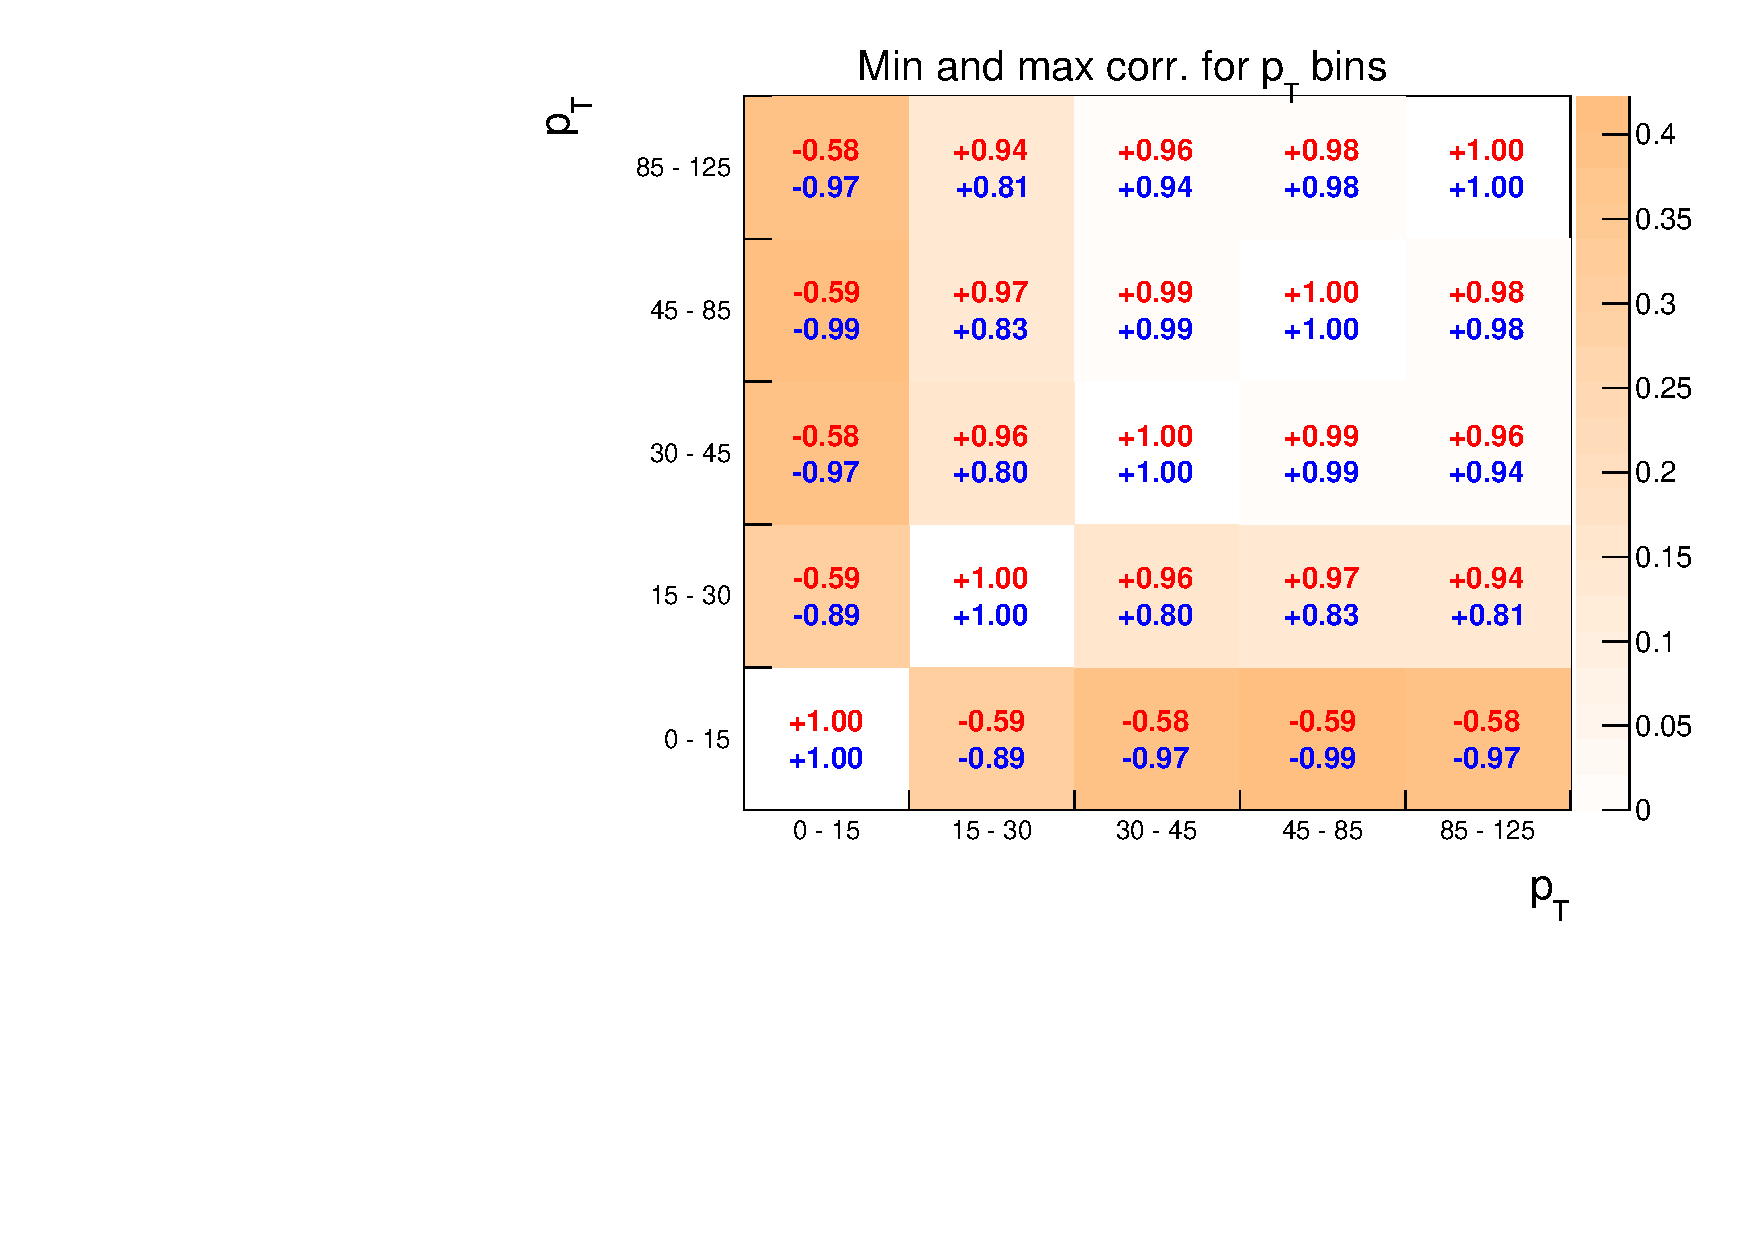
\includegraphics[width=\halflinewidth]{img/interpretation/other/minmax_corrMat_exp.pdf}
    \caption{
        Minima and maxima of the correlation matrices computed per coupling variation of $\kappa_b$/$\kappa_c$, for the gluon-induced contributions.
        % 
        The color scale is the difference between the minimum and maximum.
        }
    \label{fig:CorrelationMatrix_minmaxStudy}
  \end{center}
\end{figure}


% ____________________________________________________________________________
% Branching fractions

\subsubsection{Branching fractions}

The branching ratios are subject to uncertainties stemming from the input parameters ($\alpha_s$, $m_b$, $m_c$ and $m_t$) and theoretical uncertainties due to missing higher order contributions.
% 
The theoretical uncertainties are assumed to be uncorrelated, whereas the parametric uncertainties are assumed to be fully correlated.
% 
Uncertainties on the partial widths are taken from Ref.~\cite{deFlorian:2016spz}.
% 
Figure~\ref{fig:scans_kappatkappag_brcomparison} shows the $\kappa_b$/$\kappa_c$ with branching ratios fixed to their SM expectation, with and without the uncertainties on the branching ratios.
% 
The difference is clearly negligibly small, and as such the uncertainties on the branching ratios are neglected in further results.


\begin{figure}[hbtp]
  \begin{center}
    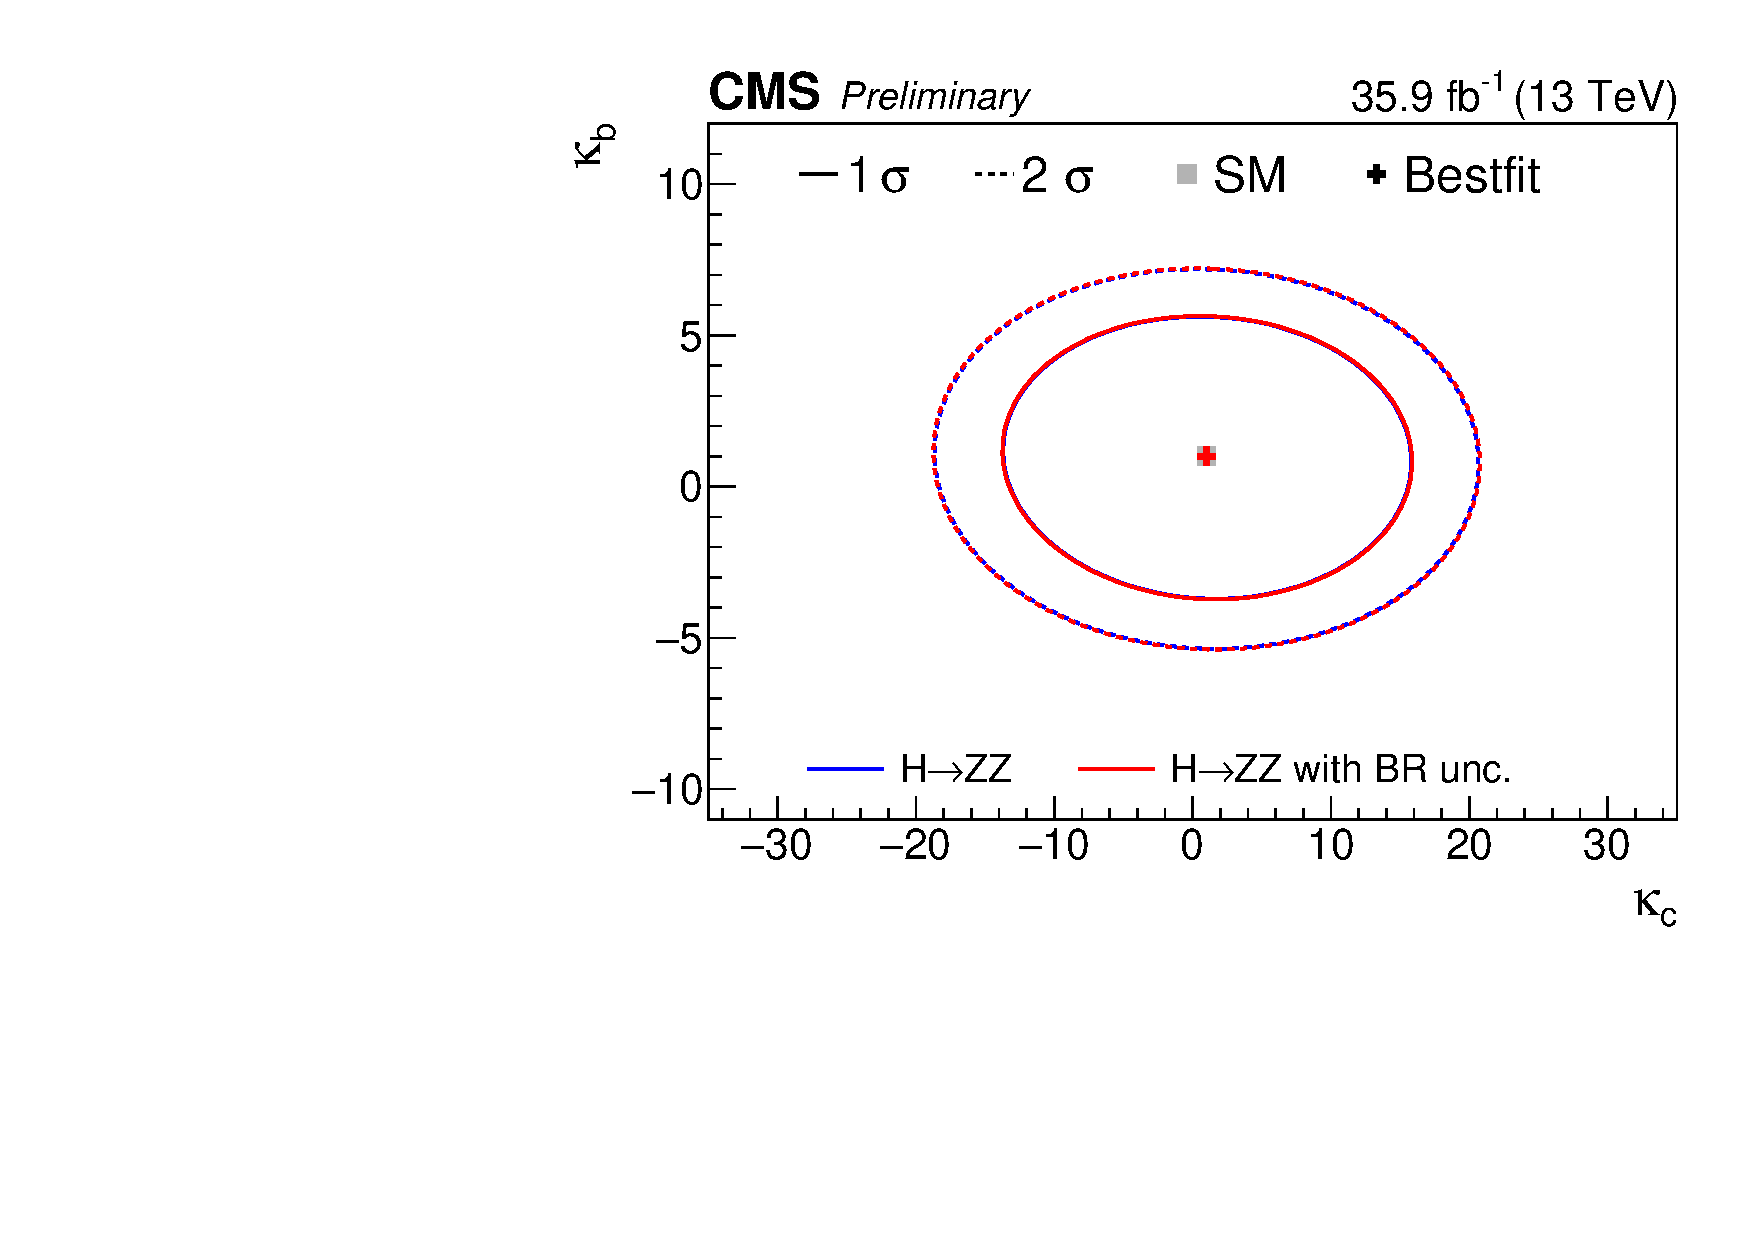
\includegraphics[width=\halflinewidth]{img/interpretation/other/multicont_Yukawa_compareBRuncertainties_asimov.pdf}
    % 
    \caption{
        $\kappa_b$/$\kappa_c$ with branching ratios fixed to their SM expectation, with and without the uncertainties on the branching ratios.
        }
    \label{fig:scans_kappatkappag_brcomparison}
  \end{center}
\end{figure}

